\subsection{Trustable}
The trust between the platform that we want to use and the user has to be firm.
Therefore we will have to guarantee the protection of your privacy and give you the certainty that if
We use your data only for a specific purpose and we will make it clear,
what is that purpose, that is, transparency.
We must therefore minimize the risk of disclosing your data, that is, saving
for your safety, integrity and confidentiality.
For this we must follow both the legal norms and an ethics of good practices.
Do not force an identified if you can show information.
Always ask for permission to capture data and make clear the purpose of these.


\subsubsection{How to solve it} 
Use of secure platforms, such as SSL if we develop a web application.
If we use third-party APIs, make sure both your reputation and the level of security it offers.
Implement a system that does not allow linking the data with a user.
Give the user the possibility to delete their data if they wish.


\subsubsection{How we solve it. Aire Guru} 
In our case, security is paramount since for our star function, personal history
of exposure to contamination, it is not essential to collect the user's position.
SSL has been used to achieve a level of competent security, which guarantees the encryption of
the information sent through the network.
For the identification of the user a secure and proven API has been used, we use the identification
that Firebase provides us. This API provides us with an identifier, which can be encrypted or not.
We have of course used encryption. When the data reaches our database,
check the user and if it is correct we will re-encrypt the user with our own password to
so avoid that you can relate the database of firebase with our database.

Regarding the user's position, we never store his exact position, only the polygon where he is
and we also implemented a minimum of time. This allows us to have the necessary precision to show you your
Exposure to contaminants but not user tracking.

Following the code of good practices, you never begin to collect the user's position without their permission,
for this we need an explicit action. In our case, the user will have to select "My
"and accept that we read your position. Of course the user can always revoke this permission and
delete your data at any time from the configuration section. \\

\newpage
\begin{figure}[ht]
    \centering
   \subfigure[Location Access]
    {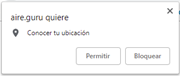
\includegraphics[width=5.5cm  ]{locationAccess}}
    \hfill
    \subfigure [Settings]
       { 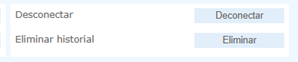
\includegraphics[width=5.5cm]{settings}}
   
  \caption{Filters}
    \end{figure}

    The collection of position data is not exhaustive, but guarantees accuracy. \\

    As we want a transparent tool, we explain to the user that we need their data before
    to be identified, and of course, the identification is optional. \\

    \begin{figure}[ht]
        \centering
        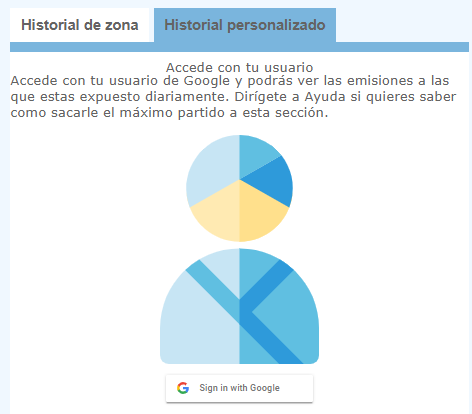
\includegraphics[width=8cm]{loginInfo}
        \caption{Info before login}
    \end{figure}

\elsparagraph{Evaluation}  
\begin{itemize}
    \done Code of good practices
    \done It is not possible to relate the identification of the firebase user with our database
    \crossed Some users indicated that they would prefer to create an account with a username and password
         and not use your email account for fear of "information theft"
    
\end{itemize}
\newpage